\documentclass{report}
\usepackage{fullpage}
\usepackage[utf8]{inputenc}
\usepackage{setspace} 
\usepackage[ampersand]{easylist}

\usepackage{graphicx}
\graphicspath{{images/}}

\usepackage{color}
\usepackage{listings}
\lstset{ %
language=C++,                % choose the language of the code
basicstyle=\footnotesize,       % the size of the fonts that are used for the code
numbers=left,                   % where to put the line-numbers
numberstyle=\footnotesize,      % the size of the fonts that are used for the line-numbers
stepnumber=1,                   % the step between two line-numbers. If it is 1 each line will be numbered
numbersep=5pt,                  % how far the line-numbers are from the code
backgroundcolor=\color{white},  % choose the background color. You must add \usepackage{color}
showspaces=false,               % show spaces adding particular underscores
showstringspaces=false,         % underline spaces within strings
showtabs=false,                 % show tabs within strings adding particular underscores
frame=single,           % adds a frame around the code
tabsize=2,          % sets default tabsize to 2 spaces
captionpos=b,           % sets the caption-position to bottom
breaklines=true,        % sets automatic line breaking
breakatwhitespace=false,    % sets if automatic breaks should only happen at whitespace
escapeinside={\%*}{*)}          % if you want to add a comment within your code
}

%\singlespacing 
%\onehalfspacing 
%\doublespacing 
%\setstretch{1.1}
\renewcommand{\baselinestretch}{2}
\author{Nicolas Tollenaere}
\title{Rapport de stage de fin d'études : Évaluation et prédiction du partage des ressources mémoires
dans un programme multitâches}
\begin{document}
\maketitle
\tableofcontents




\chapter{Introduction}
Ce document rapporte mon activité durant le stage de fin d'études que j'ai 
realisé a l'Inria, l'Institut National de Recherche en Informatique et
Automatique, au sein de l'équipe CORSE (Compilation and Optimisation in Runtime).
J'ai donc eu affaires naturellement à des problématiques de recherche mais aussi à
des problématiques d'ingénierie tout au long de ces six mois. Plus précisément, mes travaux ont été
liées à des problématiques de programmation concurrente et multithreadée. Il s'est agi au départ d'évaluer
le comportement et le partage des ressources sur des architectures dites NUMA, Non-Uniform Memory Access. 
La problématique a ensuite évolué, pour des raisons que l'on verra, vers des questions de partage de cache
entre différents threads.
En l'état, mon travail a consisté en la réalisation d'un benchmark permettant d'évaluer les performances
d'une architecture lorsque qu'un ou plusieurs threads sont limités et se disputent des ressources mémoire.
On expliquera ici les difficultés qui ont été rencontrées et comment ces difficultés ont pu être dépassées.
La problématique a ensuite été d'essayer de parvenir à proposer des algorithmes pertinents pour réaliser 
des prédictions quant aux comportements des threads en concurrence. 
Plusieurs pistes et modèles ont été explorés, certains résistant mieux que d'autres aux vérifications 
expérimentales.
Après avoir rappelé le contexte du stage, le statut de l'INRIA, les thèmes de travail de l'équipe CORSE où
j'ai été intégré, nous allons voir en détail toutes les étapes qui ont été rencontrées au cours de ce stage. 
Nous remettrons ensuite en perspective ces travaux et l'intérêt qu'ils peuvent représenter dans les 
domaines traités par l'équipe.

\chapter{Le contexte}
\section{L'entreprise}

Inria est l'Institut National de Recherche en Informatique et Automatique. Créé en 1967, il a le statut
d'établissement à caractère scientifique et technologique. Sa mission est de coordonner la recherche dans 
les domaines liés à l'informatique au niveau national. Il promeut, comme on peut le trouver sur le site officiel,
l'excellence scientifique au service du transfert technologique et de la société.
\\ Depuis sa création, Inria a développé de nombreux projets scientifques qui font jusqu'à aujourd'hui 
sa réputation.  On peut citer, parmi les projets les plus connus , ses travaux sur les développements 
d'internet, les langages de programmations Caml, Caml Light et Ocaml , le logiciel de calcul scientifique 
Scilab, l'assistant de preuve Coq ou la bibliothèque de calcul flottant en haute précision GNU MPFR.
\\ Inria emploie aujourd'hui 2700 collaborateurs, issus des structures françaises mais aussi des universités
du monde entier. De par ses nombreux partenariats et son rayonnement dans la sphère scientifique de 
l'informatique, il est un acteur majeur de la recherche au niveau mondial.
Inria est également reconnu pour son implication active dans la promotion du logiciel libre. Ainsi, les
projets Ocaml, Coq, Scilab ou GNU MPFR sont tous déposés sous licence libre, soit directement sous la 
licence GNU GPL, soit sous la licence compatible créée par Inria en collaboration avec le CEA et le CNRS
 CeCILL (CEA CNRS Inria Logiciel Libre). La bibliothèque MPFR (Multiple Precision Floating Point Reliably)
 est d'ailleurs utilisée dans le célèbre compilateur GNU GCC (GNU Compiler Collection).
\\ Les effectifs de l'Inria sont organisées en de nombreuses équipes constituées en moyenne d'une vingtaine
 de personnes (membres permanents ou non-permanents), accueillant à l'occasion (ou même de manière continue)
des chercheurs dépendants d'autres institutions. Les équipes sont à leur tour réparties sur huit centres 
autonomes dispersés sur tout le territoire métropolitain. C'est dans l'une de ces équipes que j'ai réalisé
mon stage de fin d'études.

\section{L'équipe}

Au sein de l'équipe Inria Rhones-Alpes, sur un site détaché dans les locaux de Minatech 
et du CEA de Grenoble, je suis intégré au sein de l'équipe CORSE (Compiler Optimization 
and Runtime SystEm). Créée il y a cinq ans, cette équipe est dirigée par Fabrice RASTELLO.
Comme son nom l'indique, elle s'occupe de problèmes liés à l'interaction entre la compilation
et l'exécution d'un programme, ainsi que d'autres problématiques connexes comme le déboguage.
Elle rassemble aussi bien des personnes spécialistes de la compilation que des spécialistes 
du runtime (donc de l'exécution).
\\ La conception et les perspectives des architectures matérielles ont beaucoup évolué dans les 
quinze dernières années.  Des tout débuts de l'informatique jusqu'au début des années 2000 
environ, les différents processeurs et composants ont eu tendance à converger et à se faire de
plus en plus puissantes (on parle ici de fréquence des processeurs et de nombres d'instructions 
par seconde). On imaginait généralement que cette évolution se poursuivrait et que conséquemment, 
un même programme pourrait être exécuté plus rapidement dès lors qu'on le ferait tourner sur une 
nouvelle architecture. Les années 2000 ont mis fin à cette croyance lorsque des problématiques 
telles que la consommation d'électricité ainsi que le dégagement d'énergie et de chaleur qui 
s'ensuivait et qui posait de gros problèmes quant au refroidissement du matériel sont apparus. Il 
était devenu impossible d'augmenter la puissance de calcul brute des processeurs sans détériorer 
très considérablement leur consommation d'énergie, mais aussi probablement leur durée de vie au vu du 
problème de refroidissement. Sur un tout autre plan, s'est posée la question de ce que l'on a 
appelé le Memory Gap.  Au début de l'informatique, les architectures avaient généralement une capacité
de calcul inférieure à leur capacité à rapatrier des données depuis la mémoire. Ainsi, la puissance de
calcul d'un programme se trouvait très souvent limitante par rapport à sa capacité de chargement. 
L'évolution de la technologie s'est faite de telle manière que le rapport se trouve aujourd'hui 
être inversé, c'est-à-dire que réaliser une opération simple sur une ou plusieurs données (une addition
ou une multiplication par exemple) est beaucoup plus rapide que de rapatrier cette ou ces données depuis
la mémoire principale. Dès lors, augmenter encore cette puissance de calcul peut se trouver tout à 
fait inutile dans de nombreux cas dans la mesure où bien des programmes passeront plus de temps à 
attendre l'arrivée des données qu'à réellement effectuer des calculs dessus. 
\\ Ces considérations ont rendu déraisonnable l'idée de continuer à augmenter indéfiniment la fréquence des 
processeurs. Il s'ensuivit que les architectures recommencèrent à se diversifier pour pouvoir continuer à 
offrir des performances accrues. On observe ainsi une recrudescence de machines très spécialisées, par 
exemple dans le traitement d'image (les cartes graphiques) ou dans la cryptographie. Par ailleurs, les 
architectures dites parallèles ainsi que distribuées connurent et connaissent toujours un développement 
significatif.
\\ Dans ce contexte, les problématiques de compilation et d'exécution deviennent cruciales, car un même 
programme sémantique doit être adapté de manière efficace à des cibles très diverses. Il est parfois 
très difficile, par exemple, d'exécuter de manière efficace sur une machine parallèle un programme
prévu à l'origine pour une exécution séquentielle (il est même souvent nécessaire de repenser 
entièrement le programme). Dans l'idéal, il faudrait que le programmeur n'ait en aucun cas à gérer des 
questions spécifiques à chaque architecture, à la fois dans un souci de simplicité et de portabilité.
Il serait donc souhaitable que cette charge soit entièrement dévolue au compilateur, qui lui est 
capable de cibler spécifiquement un environnement d'exécution. En pratique, tout ceci est généralement 
assez compliqué. Le travail de l'équipe se situe ici. Les membres cherchent à fournir des outils
permettant de tirer le meilleur parti d'architectures très différentes à partir d'un même code source, 
selon des métriques qui peuvent également varier avec la situation. Il s'agit généralement d'améliorer 
la performance en temps, en espace mémoire et/ou en énergie.
\\ Pour cela, l'équipe développe, pour une part, des stratégies dynamiques où les décisions sont prises au
moment de l'exécution réelle du programme sur une machine. Ces décisions peuvent concerner l'équilibrage
des charges, la répartition des tâches sur différents processeurs, etc.
\\Pour une autre part, l'équipe développe aussi des stratégies statiques, dans lesquelles les décisions
sont prises au moment de la compilation du programme. De nombreuses optimisations peuvent être réalisées
à ce moment-là grâce à une analyse du code (par exemple l'élimination de code mort, l'inlining de fonction
ou l'élimination des variables intermédiaires).
\\Mais surtout, l'équipe cherche autant que possible à développer des tactiques améliorant l'interface
entre les deux. D'un côté, le système runtime (dynamique) dispose d'informations précieuses sur 
l'environnement dans lequel le programme est exécuté. Par contre, il n'a qu'une vision partielle et 
immédiate de ce programme, puisqu'il ne peut en réaliser une analyse globale. D'un autre côté, le 
compilateur, s'il n'a pas d'informations sur le contexte précis d'exécution, réalise néanmoins une
analyse globale du code. On peut donc imaginer que le compilateur pourrait passer des informations 
utiles pour guider le runtime dans sa prise de décision.
\\Les domaines d'applications spécifiques de ces travaux sont nombreux mais ont trait essentiellement
au calcul scientifique. Des programmes liés à la physique des matériaux ou à la propagation d'ondes
ont directement tiré profit des travaux de l'équipe. Il arrive également que des partenariats se
fassent avec des fabricants de processeurs ou d'autres composants afin de réaliser un travail spécifique
d'optimisation sur leurs machines.
\section{Mon stage}
Au sein de l'équipe Corse, je suis co-encadré par Florent Bouchez-Tichadou, maître de conférence, ainsi
que par Fabrice Rastello, directeur de recherche et chef de l'équipe. L'idée de départ du stage est de 
s'intéresser à des problématiques liées à la bande-passante mémoire. Au vu des directions de recherche
de l'équipe, le choix de s'intéresser à la technologie OpenMP était relativement naturel. C'est donc
 ce que j'ai fait dans la première partie de mon stage.
\chapter{Première partie du stage : OpenMP et Numa}

Ma mission était initialement liée à la technologie OpenMP. OpenMP est une interface de programmation
disponible pour les langages C, C++ et Fortran qui permet de faciliter grandement l'écriture de programmes
parallèles. Comme nous allons le voir, elle fait intervenir à la fois des techniques de compilation et des
techniques dynamique, ce qui la place au coeur des thèmes de l'équipe. L'idée était d'étudier le 
d'applications utilisant OpenMP sur des architectures particulières. Les machines ciblées étaient de type
Non Uniform Memory Architecture. Cela signifie que si chaque processeur a accès à toute la mémoire de la
machine, il a néanmoins un accès privilégié à une certaine portion de cette mémoire (on parle de noeud) et
met donc plus de temps à accéder à une donnée stockée dans un autre noeud. Il peut donc y avoir des cas où
des threads se trouvent obligés d'accéder à une mémoire distante, ce qui aurait peut-être pu être évité. 
Nous allons donc maintenant :
\begin{easylist}[checklist]
   & expliquer plus précisément le fonctionnement d'OpenMP 
   & détailler la raison d'être et les enjeux des architectures NUMA
   & montrer l'avancée dans le stage, les solutions déjà existantes et la démarche
   & montrer ce qui nous a poussé à faire évoluer le sujet de travail 
  \end{easylist}
  \section{OpenMP : fonctionnement}
OpenMP signifie Open Multi-Processing. Il s'agit, comme nous l'avons précisé précédemment, d'une interface 
de programmation pour les langages C, C++ et Fortran. OpenMP est géré par un consortium, the OpenMP 
Architecture Review Board. Plus précisément, ce consortium produit une spécification d'OpenMP, donc une 
liste des comportements et des options auquels un utilisateur peut s'attendre en utilisant OpenMP.
\\Il existe ensuite différentes implémentations, qui pourront remplir en totalité ou partiellement la 
dernière version ou une version plus ancienne de la spécification OpenMP. Chaque entreprise, groupe 
ou entité qui voudrait mettre à disposition sa version d'OpenMP a, même s'il compte respecter à la lettre
la spécification, une marge de manoeuvre très importante quant à la ``machinerie interne'' de 
l'application. Certains pourront décider notamment d'optimiser leur implémentation pour un type 
d'architecture particulière, et pourquoi pas de fournir des outils supplémentaires au programmeur. Il 
est d'ailleurs arrivé que certains de ces outils se retrouvent ensuite dans une version ultérieure 
de la spécification.
\\Nous allons d'abord évoquer OpenMP d'un point de vue utilisateur, afin de donner une meilleure idée 
de ce qu'il peut apporter. Nous rentrerons ensuite dans les détails techniques de l'implémentation, 
ce qui permettra de montrer en quoi cette technique fait intervenir une interaction entre la compilation
et l'exécution.

\subsection{Utilisation}

L'intérêt d'OpenMP est de faciliter l'écriture de programmes parallèles. Plus que cela, il s'agit aussi 
de rendre ces programmes plus portables en permettant au codeur de s'abstraire de paramètres comme le 
système d'exploitation de la machine cible (bien qu'il existe des librairies standards de multithreading, 
de nombreuses fonctionnalités avancées comme l'association d'une tâche à un cpu particulier restent encore
spécifiques à l'OS), ou le choix du nombre de threads approprié, qui dépend de l'architecture.
\\L'idée générale est de préciser les régions du code que l'on souhaite exécuter en parallèle. En C et 
C++, cela se fait au moyen de pragmas. Il s'agit de directives adressées au compilateur, sur des lignes qui 
commencent par la chaîne \#pragma omp. Une région signalé par un \#pragma omp parallel sera 
exécutée autant de fois qu'il y aura eu de threads créés par le runtime. Ce nombre correspond généralement 
au nombre de coeurs de la machine sur laquelle le programme est exécuté. Ainsi, dans le programme 
ci-dessous, Hello World sera affiché quatre fois si la machine possède quatre coeurs.
\begin{lstlisting}
#include <stdio.h>
#include <omp.h>

int main(void)
{
    #pragma omp parallel
    printf("Hello, world.\n");
    return 0;
}


\end{lstlisting}

Il faut simplement ajouter une option de compilation (fopenmp pour gcc et clang) pour compiler
correctement le programme.
De nombreuses autres possibilités sont offertes dans la mesure où les programmes concurrents ont
généralement besoin de synchronisation. Ainsi OpenMP fournit-il notamment des barrières (\#pragma
omp barrier) qui permettent d'imposer aux threads un point de synchronisation. Chaque thread se voit 
attribué un identifiant, ce qui permet de différencier les tâches selon les threads. Il est aussi
possible de faire en sorte qu'une portion du programme ne soit accomplie que par le ``master''
(\#pragma omp master - le master est simplement le thread qui possède l'id 0), d'exiger que cette
portion ne soit accédée que par un thread à la fois, voire par un seul thread, peu importe lequel.
Ainsi, considérons l'exemple suivant : 
\begin{lstlisting}
#include <stdio.h>
#include <omp.h>

int main(void)
{
#pragma omp parallel
  {
    int tid = omp_get_thread_num();
    printf("Hello, world from thread \%d\n", tid);
#pragma omp master
    printf("I'm the master ! \n" );
  }
}
\end{lstlisting}
Une sortie typique de ce programme serait, par exemple :
\\Hello, world from thread 2
\\Hello, world from thread 0
\\Hello, world from thread 1
\\Hello, world from thread 3
\\ I'm the master ! 

Mais il est aussi possible d'avoir :
\\Hello, world from thread 2
\\Hello, world from thread 0
\\ I'm the master ! 
\\Hello, world from thread 1
\\Hello, world from thread 3

 L'instruction barrier nous permet d'éviter cela.
\begin{lstlisting}
#include <stdio.h>
#include <omp.h>

int main(void)
{
#pragma omp parallel
  {
    int tid = omp_get_thread_num();
    printf("Hello, world from thread \%d\n", tid);
#pragma omp barrier
#pragma omp master
    printf("I'm the master ! \n" );
  }
}


\end{lstlisting}

De la sorte, on a contraint le programme à afficher I'm the master seulement une fois que chacun 
des threads aura affiché son Hello.

La politique de partage de ressources entre les threads est également un élément clé de la programmation
concurrente. Conséquemment, OpenMP offre la possibilité de déclarer une variable ``shared'' ou ``private''.
Dans le premier cas, elle sera visible et modifiable par tous les threads, et son accès nécessitera sans
doute une synchronisation. Dans le second cas, chaque thread aura une copie de la variable invisible aux 
autres. Il existe des variations que nous n'allons pas discuter.
\\Il n'est pas utile de rentrer ici plus longuement dans les détails. Ajoutons simplement que la
norme a bien entendu énormément évolué au cours du temps pour répondre à des besoins de plus en plus
variés. Ainsi, il est désormais possible de réaliser des parallélisations vectorielles. Des possibilités
ont également été ajoutées pour pouvoir changer à loisir le nombre de threads engagés ainsi que le coeur 
sur lequel ils s'exécuteront. Voyons maintenant comment se déroule concrètement la compilation et
l'exécution d'un programme OpenMP.

\subsection{Fonctionnement}

La spécification OpenMP jouit de nombreuses implémentations. Deux sont particulièrement notables : celle
qui est fournie avec GCC (Gnu Compiler Collection) et celle développée Intel, utilisée en particulier
par Clang. Cependant, il en existe d'autres, dont certaines sont même développées à l'Inria, comme Kaapi
ou StarPU.
\\Il convient maintenant de mieux préciser le fonctionnement d'une implémentation OpenMP. Celui-ci est
divisé en deux parties : une part du travail est réalisée à la compilation. En se basant sur les pragmas
écrites par le programmeur, le compilateur va isoler dans le code les portions destinées à être exécutées
en parallèle, et effectuer quelques autres transformations. 
\\ La deuxième partie du travail sera effectuée directement à l'exécution par un système runtime. À ce 
moment seront déterminés des paramètres tels que le nombre de threads. Il faut bien comprendre que si les
deux parties sont bien distinctes, elles sont néanmoins fortement interdépendantes : en règle générale,
un programme compilé avec un compilateur donné ne pourra fonctionner qu'avec le runtime correspondant,
même si cette limitation est contournable. Cela explique pourquoi les deux implémentations majeures ont
été développés par des entités fortement impliquées dans le domaine de la  compilation, à 
savoir GCC et Intel. 
\\Voyons un peu plus en détails chacun des deux points, en commençant par la compilation. Comme dit plus
haut, l'idée ici est d'isoler le code à paralléliser du reste et d'introduire au bon endroit des appels
aux fonctionnalités appropriées du runtime. Pour cela, le compilateur réalise une opération
d'``outilining''. Comme le nom l'indique, il s'agit de l'exact inverse de l'inlining. Là où l'inlining
prend le code d'une fonction pour l'injecter à l'endroit où la fonction en question est appelée, 
l'outilining sélectionne une portion du code et la remplace par un appel à une fonction comprenant le
code correspondant. On supprime une indirection dans le premier cas là où on en rajoute une dans le 
second. Ainsi, le code suivant :
\begin{lstlisting}
#include <stdio.h>
#include <omp.h>

int main(void)
{
    #pragma omp parallel
    printf("Hello, world.\n");
    return 0;
}


\end{lstlisting}

pourra être remplacé par celui-ci :
\begin{lstlisting}
#include <stdio.h>
#include <omp.h>

void omp_outlined_fun()
{
    printf("Hello, world.\n");
}

int main(void)
{
  omp_outlined_fun();
    return 0;
}



\end{lstlisting}
Le nom de la fonction choisi ici est un exemple : il dépend du compilateur utilisé. Cette opération est
de toute façon transparente pour l'utilisateur. 
\\L'outlining seul ne suffit pas : l'objectif concret est d'indiquer au runtime sur quelle partie du code
il est censé travailler. Pour cela, la fonction qui a été outlinée va en fait être passée en paramètre
(sous forme d'un pointeur) à une fonction de la bibliothèque du runtime. Pour le runtime d'Intel, la 
fonction d'entrée s'appelle kmpc\_fork\_call. On aura donc, schématiquement : 

\begin{lstlisting}
#include <stdio.h>
#include <omp.h>

void omp_outlined_fun()
{
    printf("Hello, world.\n");
}

int main(void)
{
    kmpc_fork_call((void (void)*)omp_outlined_fun);
    return 0;
}

\end{lstlisting}

D'autres arguments sont également passés à la fonction. Pour ce qui est des variables, un pointeur est
passé en argument de la fonction outlinée si elle est partagée, ou la variable est placée directement
dans la pile (elle est donc déclarée au début du corps de la fonction) quand elle est privée.
\\Tout marche grossièrement de cette manière : les différentes directives passées au travers des pragmas
sont associés à des fonctions du runtime auxquelles des appels sont faits dans le programme produit par
le compilateur. 
\\Quant au runtime, il s'agit en fait simplement d'une bibliothèque dynamique. Cette bibliothèque 
contient toutes les fonctions évoquées au-dessus. Comme la bibliothèque est dynamique, le linkage est fait
au moment de l'exécution plutôt qu'au moment de la compilation, ce qui autorise un programme à utiliser
des versions plus récentes que celles qui existaient lorsqu'il a été compilé (pour peu qu'on ait assuré
la rétrocompatibilité de la bibliothèque). Il faut cependant que le compilateur connaissent la signature
(nom et type des arguments) des fonctions utilisées. C'est la raison de la dépendance runtime/compilateur
déjà évoquée. Comme on l'a dit, cette limitation peut néanmoins être contournée. Ainsi, le support 
d'exécution d'Intel peut exécuter des programmes compilés avec gcc. Pour cela, il inclue dans son code
des redirections des fonctions du runtime de gcc vers les fonctions de son propre runtime. Néanmoins,
ceci n'est pas généralisable.
\\C'est à peu près tout ce que l'on peut dire du fonctionnement d'OpenMP sans rentrer dans des détails
propres à une implémentation particulière. Quand bien même la contrainte de la spécification induit des
similitudes dans les codes, on trouvera presque partout des spécificités plus ou moins marquées. Il peut
d'ailleurs arriver que deux implémentations produisent des performances différentes en fonction des
situations. Nous verrons tout cela un peu plus loin, lorsque l'on étudiera plus particulièrement
le fonctionnement de Clang dans la situation qui nous intéresse.

\section{Les architectures NUMA}
NUMA signifie, comme nous l'avons déjà précisé auparavant, Non-Uniform Memory Architecture. Ces 
architectures possèdent généralement de nombreux coeurs. Leur spécificité est que si ces coeurs 
peuvent accéder à l'intégralité de la mémoire de la machine, ils ne disposent pas d'un accès uniforme : 
ils sont rassemblés en groupes (par exemple de huit coeurs) qui ont chacun un accès privilégié à une 
portion de la mémoire. L'ensemble groupe de coeurs/portion de la mémoire privilégiée est appelé un 
noeud. Ainsi, un coeur accèdera plus rapidement à une donnée située dans son noeud qu'à une donnée 
située ailleurs. La figure \ref{fig:NUMA1} montre ce fonctionnement. L'accès à un noeud distant 
est plus long car il nécessite une requête du réseau interconnectant les noeuds.

\begin{figure}
  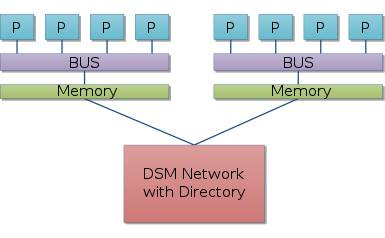
\includegraphics[width=\linewidth]{NUMA.jpg}
  \caption{schéma simplifié d'une architecture NUMA}
  \label{fig:NUMA1}
\end{figure}

Les architectures NUMA ont commencé à être étudiées, produites et vendues comme des réponses au problème
du memory gap évoqué plus haut. Pour rappel, le memory gap désigne l'écart croissant entre les performances
de calcul et les performances de bande-passante mémoire des architectures, les dernières étant désormais 
largement dépassées par les premières. Dans le cas d'une architecture disposant de très nombreux coeurs,
l'accès à la mémoire peut très vite devenir problématique dans la mesure où chacun des coeurs partagent
les mêmes ressources pour récupérer leurs données. Ainsi, si beaucoup de coeurs essaient d'accéder en
même temps à la mémoire, le temps d'accès par coeur se trouvera très dégradé, au point que l'augmentation
du nombre de coeurs deviendra contre-productive. 
\\Ce problème peut être mitigé avec les architectures NUMA. En séparant la mémoire en différents noeuds,
on essaie de diminuer les cas où plusieurs coeurs entreront en concurrence pour la même ressource. Dans
le cas idéal où chaque coeur n'accède qu'à des données situées sur son noeud, on garantit que jamais
plus de huit coeurs (si le noeud en contient huit) ne se partageront le réseau. Bien entendu, si les
coeurs commencent à beaucoup accéder à des données situées sur des noeuds distants, le problème se posera
à nouveau. Les politiques d'allocation mémoire sont conçues pour éviter au maximum ce genre de configuration.
Le système est plus flexible qu'un simple cluster dans la mesure où la communication de données entre noeuds
est transparente d'un point de vue logique - la différence ne se fait que sur le temps de transfert, là
où un système par messages, type MPI,  serait nécessaire pour un cluster. NUMA est donc un compromis 
considéré comme acceptable entre un système multicoeurs à mémoire partagée uniforme et un cluster.

\section{Avancées pendant le stage}
L'idée de base est d'observer l'interaction entre OpenMP et les architectures NUMA. Plus explicitement,
on veut savoir comment se déroule l'exécution d'un programme OpenMP sur une machine NUMA, et si 
éventuellement des comportements non-optimaux peuvent se produire, à savoir est-il possible qu'un thread
se trouve accéder à un noeud NUMA distant. Si la réponse est affirmative - et si le cas se produit 
suffisamment souvent pour être considéré comme pathologique - peut-on améliorer la situation ?
\\OpenMP ne gère jamais l'allocation des données en mémoire. De fait, les programmes reposent sur 
l'implémentation présente en local de fonctions comme malloc ou calloc, ou même à plus bas niveau
d'appels systèmes comme mmap. Une partie de mon travail a consisté à décrypter les interactions
entre chacun de ces composants : quand un programme s'éxécutant sur un cpu donné alloue une variable,
à quel moment et dans quelle partie de la mémoire elle sera réellement enregistrée ? Il m'a également fallu
décrypter le fonctionnement du support d'exécution OpenMP et notamment sa tactique quant à la migration de
tâches (un problème que nous allons expliquer ensuite). Enfin, une partie importante était de réaliser des 
benchmarks pour évaluer les pertes éventuelles dues à des accès à une mémoire distante. 
\\J'ai eu accès, dans le cadre de mes travaux, à une architecture NUMA appartenant à l'université de 
Grenoble. Cette machine, appelée Idchire, dispose de 192 coeurs répartis sur 24 noeuds NUMA distincts. 
C'est sur cette machine que j'ai réalisé les expériences que je décris dans cette partie.

\subsection{Politique d'accès mémoire sur une machine NUMA}

Comme nous l'avons dit, l'allocation des données en mémoire est indépendante du support d'exécution OpenMP.
Néanmoins, une connaissance claire de cette politique, de l'endroit et du moment où une donnée sera écrite
en mémoire est nécessaire si l'on veut appréhender comment les mécanisme d'OpenMP vont interagir avec ce
problème. Pour profiter de l'architecture NUMA, l'implémentation d'une politique spécifique est bien 
entendu requise : il faut maximiser la localité des données et faire en sorte que les accès locaux soient
la norme plutôt que l'exception. 
\\Commençons par faire un rappel sur le système de mémoire virtuelle des systèmes d'exploitations modernes.
Les premiers ordinateurs laissaient leurs programmes accéder directement à la mémoire physique de leur
système. Cela posaient de nombreux problèmes, le plus important étant celui de l'isolation des processus.
Ainsi, un programme avait la possibilité de modifier les données d'un programme voisin. Ceci représentait
une faille de sécurité majeure, dans la mesure où des programmes importants pouvaient se trouver invalidés
par le travail d'un processus annexes. Une attention toute particulière devait être accordée aux accès 
à la mémoire.
\\Pour remédier à ce problème, les informaticiens ont inventé dans les années 1960 le principe de la 
mémoire virtuelle. La mémoire physique est divisée en ``blocs'' d'une taille donnée qu'on appelle
des pages. Lorsqu'il souhaite obtenir de la mémoire, un processus va en faire la demande au système
d'exploitation, par le biais d'un appel système comme mmap. Dans l'hypothèse où il possède la mémoire 
disponible, celui-ci va alors lui attribuer un nombre de pages contenant la quantité de mémoire 
demandée. Un autre processus ne pourra, sauf appel à un mécanisme spécifique de partage de mémoire, 
accéder aux données stockées dans ces pages, réglant ainsi la question de l'isolation mémoire. Le 
système de mémoire virtuelle présente d'autres avantages, dont celui de pouvoir utiliser la mémoire 
de masse (comme un disque dur) comme extension de la mémoire vive par un mécanisme de swap : dans 
la situation où plus de pages sont attribuées qu'il n'y a de place disponible en mémoire vive, les 
pages surnuméraires sont déplacées vers le disque dur, puis rapatriées lorsque les programmes veulent
y accéder. Dans la mesure où l'accès au disque dur est plus lent que l'accès à la mémoire principale,
ce mécanisme a un impact fort sur la performance.
\\Pour pouvoir associer une adresse virtuelle et une adresse physique, on maintient une table des 
pages qui retient donc l'emplacement d'une page donnée en mémoire physique ainsi que l'identité
du processus propriétaire de chacune des pages. C'est le rôle de la MMU (Memory Management Unit),
une des composantes de l'architecture matérielle. La table des pages est stockée en mémoire, mais
une partie est maintenue dans un cache spécifique appelé le TLB (Translation Lookaside Buffer).
\\Le système de pages pose la question du choix de la taille de page appropriée. Une page trop petite
oblige les processus à faire très souvent appel au système d'exploitation et donc à déclencher un
``context switch'', ce qui est coûteux en terme de performance. D'un autre côté, une page trop large
va entraîner une forte fragmentation de la mémoire, dans la mesure où beaucoup de processus 
n'utiliseront qu'une petite fraction de l'espace qui leur aura été attribué. Le choix de la taille
de pages est donc le résultat d'un compromis entre ces deux facteurs. Aujourd'hui, une page est 
typiquement constituée de 4 Kibioctets par défaut. Cependant, la plupart des architectures propose
la possibilité d'utiliser des pages plus grandes, parfois de plusieurs mebioctets ou même d'un ou
plusieurs gibioctets. Cette option est désignée par le terme ``huge pages''.
\\Revenons aux architectures NUMA. Dans une architecture uniforme classique, l'emplacement d'une
page en mémoire ne fait pas de différence dans la mesure où l'accès à la mémoire est partout identique.
Comme on l'a déjà expliqué, il n'en va pas ainsi pour une architecture NUMA où l'accès local est plus
rapide. La politique de choix de l'emplacement de la page est gérée par l'appel système et dépend
donc de l'implémentation de celui-ci, qui va bien entendu varier selon les systèmes d'exploitation.
Cependant, le principe général est le suivant : les pages sont allouées selon une politique ``paresseuse''
dite ``first touch''. Une allocation mémoire n'est pas faite au moment de l'allocation proprement dite
(c'est-à-dire de l'appel à malloc) mais seulement au moment où cette donnée sera accédée pour la première
fois. On délaie ainsi au maximum le travail proprement dit d'allocation. Cela permet aussi, dans 
l'hypothèse où le programmeur aurait alloué plus d'espace qu'il n'en utilise réellement, de ne payer que
pour les données réellements accédées. Dans le cas d'une machine NUMA, on apporte la garantie supplémentaire
que la page demandée sera allouée sur le noeud du processeur qui a réalisé le premier accès à la variable.
On espère ainsi faire en sorte que les données soient allouées sur les noeuds où elles seront le plus
souvent accédés.
\\J'ai cherché à vérifier ce qu'il en était sur la machine que j'avais à disposition. Il existe une fonction
bas niveau permettant, selon les paramètres, de déplacer une page vers un noeud donné, ou encore d'obtenir 
le noeud sur lequel cette page se trouve au moment de l'appel : il s'agit de move\_pages. Ainsi l'appel
suivant :

\begin{lstlisting}
#include <stdio.h>
#include <stdlib.h>
#include <numaif.h>
#include <unistd.h>
#include <hwloc.h>

int main()
{
	int *ptr;
	intptr_t  ptr_align;

	// get page size in bytes
	int psize = getpagesize();
	ptr = malloc(25*sizeof(int));
	*ptr = 4;
	// align pointer on page boundaries
	ptr_align = (intptr_t)ptr & ~(psize - 1);
	// move_page returns 0 in case of success
	// and set status to the node number where 
	// ptr is located when fourth argument
	// is NULL
	if ( move_pages(0, 1, (void **)&ptr_align, NULL, status, 0) == 0)
		printf("memory is at node %d\n", status[0]);
	return 0;
}

\end{lstlisting}

Ce programme permet donc de connaître le noeud sur lequel se situent nos données. J'ai utilisé une bibliothèque
développé par l'Inria appelée hwloc (pour hardware locality) qui offre de nombreuses abstractions pour 
travailler à bas niveau sur des questions d'architectures (on peut ainsi récupérer des informations sur 
la machine sur laquelle le programme est exécuté, ou encore déplacer des threads ou des processus d'un coeur
à un autre). Elle m'a servi à imposer à mon programme de s'exécuter sur le CPU 0, situé logiquement sur le
noeud 0. Voici donc le programme que j'ai exécuté :

\begin{lstlisting}
#include <stdio.h>
#include <stdlib.h>
#include <numaif.h>
#include <unistd.h>
#include <hwloc.h>

int main()
{
	int *ptr;
	intptr_t  ptr_align;

	hwloc_topology_t topology;
	hwloc_cpuset_t  set1;

	//initiating locality informations
	hwloc_topology_init(&topology);
	hwloc_topology_load(topology);
	
	
	//setting process on cpu 0 with hwloc
	set1 = (hwloc_cpuset_t) hwloc_bitmap_alloc();
	hwloc_bitmap_set(set1, 0);
	hwloc_set_cpubind(topology, (hwloc_const_cpuset_t)set1, HWLOC_CPUBIND_PROCESS);


	// get page size in bytes
	int psize = getpagesize();
	ptr = malloc(25*sizeof(int));
	*ptr = 4;
	// align pointer on page boundaries
	ptr_align = (intptr_t)ptr & ~(psize - 1);
	// move_page returns 0 in case of success
	// and set status to the node number where 
	// ptr is located when fourth argument
	// is NULL
	if ( move_pages(0, 1, (void **)&ptr_align, NULL, status, 0) == 0)
		printf("memory is at node %d\n", status[0]);
	return 0;
}

\end{lstlisting}
En exécutant ce programme, j'ai eu la surprise de voir que le noeud indiqué n'était pas
nécessairement, et même rarement, le noeud 0. Le noeud semblait plutôt être
choisi aléatoirement. Je me suis d'abord demandé si la politique de first touch était 
effectivement implémentée ici. Cependant, après discussion avec d'autres membres de l'équipe,
j'ai fini par trouver l'explication. En fait, l'implémentation de malloc, avant de demander
l'allocation d'une nouvelle page, cherche logiquement à savoir si le processus ne dispose
pas déjà de la place nécessaire. Dans cette situation, une page a déjà été allouée au processus
au moment où il a été lancé, et comme elle dispose de suffisamment d'espace libre, c'est sur elle
que l'on a alloué le tableau d'entier ptr. Il faut donc faire un malloc d'un tableau suffisamment
grand pour pouvoir dépasser la capacité de la première page. C'est ce que je fais dans la version
suivante : 

\begin{lstlisting}
#include <stdio.h>
#include <stdlib.h>
#include <numaif.h>
#include <unistd.h>
#include <hwloc.h>

int main()
{
	int *ptr, * ptr2;
	intptr_t  ptr_align;
	intptr_t  ptr_align2;

	hwloc_topology_t topology;
	hwloc_cpuset_t  set1;

	//initiating locality informations
	hwloc_topology_init(&topology);
	hwloc_topology_load(topology);
	
	
	//setting process on cpu 0 with hwloc
	set1 = (hwloc_cpuset_t) hwloc_bitmap_alloc();
	hwloc_bitmap_set(set1, 0);
	hwloc_set_cpubind(topology, (hwloc_const_cpuset_t)set1, HWLOC_CPUBIND_PROCESS);


	// get page size in bytes
	int psize = getpagesize();
	// alloc first pointer and make an acces
	ptr = malloc(25*sizeof(int));
	*ptr = 4;
	// alloc second pointer and make an acces
	ptr2 = malloc(2000*sizeof(int));
	*ptr2 = 12;
	// align pointer on page boundaries
	ptr_align = (intptr_t)ptr & ~(psize - 1);
	ptr_align2 = (intptr_t)ptr2 & ~(psize - 1);
	// move_page returns 0 in case of success
	// and set status to the node number where 
	// ptr is located when fourth argument
	// is NULL
	if ( move_pages(0, 1, (void **)&ptr_align, NULL, status, 0) == 0)
		printf("memory is at node %d\n", status[0]);
	if ( move_pages(0, 1, (void **)&ptr_align2, NULL, status, 0) == 0)
		printf("memory is at node %d\n", status[0]);
	return 0;
}

\end{lstlisting}

Cette fois, si le premier tableau pointe bien un emplacement situé sur un noeud aléatoire,
le deuxième pointe bien une page située sur le noeud 0, celui qu'on attendait. On a donc
bien confirmé la politique d'allocation attendue.
\\La conséquence immédiate de ces observations est qu'un accès à des données distantes ne peut
se produire que dans le cas où un travail commencé sur un coeur donné se poursuivrait sur un autre.
On va voir dans la suite que ce cas peut se produire avec un programme OpenMP dans certaines
situations.

\subsection{OpenMP et localité des données}
On va s'intéresser ici à la manière dont un programme OpenMP va gérer la question de la localité
d'un programme - sur quel coeur ce programme va s'exécuter, est-il susceptible de migrer d'un coeur
vers un autre. On se heurte ici à une difficulté déjà évoquée auparavant : les détails de 
fonctionnement de ce genre n'étant pas mentionnés dans la spécification, ils sont spécifiques à 
chaque implémentation. Il nous faut donc maintenant choisir une implémentation particulière 
de OpenMP pour pouvoir avancer plus loin dans l'étude. On s'intéresse ici plutôt à des propriétés
de l'exécution et donc du support d'exécution OpenMP. Plusieurs choix sont possibles : le plus
classique étant l'implémentation de GCC. Autre possibilité : le support développé en open-source 
par Intel, qui a été choisi par les développeurs de Clang (le compilateur open-source lancé par
Apple) comme son support d'exécution officiel. On pourrait aussi prendre l'un des supports 
d'exécution développés par l'Inria, Kaapi et StarPU. Kaapi est tout particulièrement intéressant
dans la mesure où des membres de Corse travaillent à plein temps dessus. D'autres supports existent,
mais ils sont a priori moins intéressants.
\\Après réflexion et consultation d'autres membres de l'équipe, mon choix s'est finalement porté
sur le support d'exécution de Clang/Intel. Les facteurs décisifs ont été que ce code était 
apparemment plus facile d'entrée notamment que celui de GCC, ou que celui de Kaapi qui n'est 
pas encore suffisamment documenté. De plus, le fait que ce runtime soit d'utilisation répandue
rend plus facile de trouver de l'aide ou des renseignements sur internet. Ce choix ne nous interdit
pas d'aller regarder le fonctionnement d'autres runtime quand ils ont été spécifiquement conçus pour
les cas qui nous préoccupent.
\\Commençons par préciser la définition des termes que l'on va utiliser. En informatique, un thread
est une séquence d'instructions. Il s'agit de la plus petite séquence d'instruction qui peut être
géré de manière indépendante par un ordonnanceur. Il s'agit d'un concept proche de celui de 
processus, à une différence près : un processus possède un espace propre en mémoire virtuelle, ce
qui implique que deux processus ne peuvent interagir que par le biais d'un passage de messages.
Au contraire, un thread partage avec d'autres threads une même portion de mémoire virtuelle, ce 
qui rend possible pour deux threads de modifier la même variable. Par ailleurs, il faut distinguer
ce concept de multithreading de celui de multithreading hardware, qui est lié mais néanmoins
distinct : en termes d'architecture, le multithreading désigne la capacité d'une unité de calcul
(Central Processing Unit) à exécuter simultanément plusieurs threads logiques. Toujours en termes
d'architecture, il n'existe pas de consensus absolu pour différencier les concepts de CPU,
processeurs ou coeurs, autant de termes dont la signification peut varier selon les constructeurs
ou le contexte. On parlera surtout ici de noeud (pour les noeuds NUMA déjà évoqués au-dessus) 
ainsi que de coeur, dans le sens ``unité de calcul élémentaire'', en gardant à l'esprit que 
plusieurs coeurs peuvent partager des ressources comme des caches à différents niveaux. On se 
contentera, lorsque ce sera pertinent, de préciser quelles ressources sont partagées entre
quels coeurs, sans plus se soucier de la terminologie exacte.
\\Revenons à OpenMP et à son support d'exécution. Ce dernier se charge de créer un nombre de 
threads logiques qui lui semble approprié avant de leur répartir le travail, d'une façon que
l'on va discuter plus tard. Une remarque d'abord : le système d'exploitation a toujours la 
main sur l'ordonnancement des threads. C'est bien entendu son rôle de répartir au mieux les
ressources entre chacun des programmes essayant de s'éxécuter. Il peut donc à loisir arrêter,
redémarrer ou déplacer à tout moment n'importe quel thread en exécution. Cela peut potentiellement
poser problème même si, en pratique, les politiques d'ordonnancement sur NUMA semble éviter les 
déplacements dispensables de threads pour profiter au mieux de la localité. Cependant, les systèmes
d'exploitations, et notamment linux, offrent des outils qui permettent d'imposer à un thread logique
de rester sur un certain emplacement physique : il s'agit de la fonction pthread\_setaffinity\_np. Le
np signifie ``non-portable'' car la fonction n'est pas POSIX, mais seulement spécifique à linux.

\begin{lstlisting}[label={lst:setaff}]
#define _GNU_SOURCE

#include <pthread.h>
#include <stdio.h>
#include <stdlib.h>

int main()
{
  cpu_set_t cpuset;
  CPU_ZERO(&cpuset);
  CPU_SET(0, &cpuset);
  if (pthread_setaffinity_np(pthread_self(), sizeof(cpu_set_t), &cpuset) == 0)
    printf("successfully pinned current thread on cpu 0\n");
  return 0;
}
\end{lstlisting}
Le code présenté dans \ref{lst:setaff} donne un exemple basique de son utilisation et se contente de
déplacer et de fixer le thread courant vers le coeur 0.
\\OpenMP offre aux utilisateurs une option pour profiter de ce mécanisme. En définissant la variable
d'environnement CPU\_PROC\_BIND à true avant de lancer un programme OpenMP, on demande au runtime de 
garantir qu'un thread ne sera pas déplacé tout au long de l'exécution du programme. On met ainsi une
sécurité quant à la possibilité qu'un thread puisse être déplacé et donc avoir à accéder à des données
qu'il avait allouées sur un autre noeud. Il y a même mieux : la spécification OpenMP définit une autre
variable d'environnement, OMP\_PLACES, qui permet de fixer les threads sur des coeurs précis. Ainsi,
OMP\_PLACES={0;4} ./example forcera le programme OpenMP example à s'exécuter exclusivement sur les
coeurs 0 à 4 (exclu). Cette option, déjà présente sur les supports d'exécution de GCC et d'Intel,
est devenu une part intégrante de la spécification depuis la version 4.0.  On voit ainsi qu'un utilisateur
avisé a la possibilité de guider le runtime pour obtenir un comportement non aberrant. 
\end{document}

